\documentclass[a4paper, 11pt]{scrreprt}
%Grunddefinitionen
\usepackage[utf8]{inputenc}
\usepackage[T1]{fontenc}
\usepackage[ngerman]{babel}
\usepackage{microtype}
\usepackage{FiraSans}
\usepackage{listings}
\usepackage{graphicx}
\usepackage{xcolor}
\usepackage{wallpaper}

%%%%%%%%%%%%%%%%%%%%%%%%%%%%%%%%%%%%%%%%%%%%%%%%d%%
\usepackage[printonlyused]{acronym}
\usepackage{listings}
\usepackage{float}

%%%%%%%%%%%%%%%%%%%%%%%%%%%%%%%%%%%%%%%%%%%%%%%%%%
% listings
\lstset{basicstyle=\footnotesize\ttfamily,breaklines=true}
\lstset{stringstyle=\color{red}} % typewriter type for strings
\lstset{keywordstyle=\color{blue}\bfseries} \lstset{commentstyle=\color{green}}
\lstset{showstringspaces=true} % no special string spaces
\lstset{backgroundcolor=\color{lightgray}} %
\lstset{literate=%
  {Ö}{{\"O}}1
  {Ä}{{\"A}}1
  {Ü}{{\"U}}1
  {ß}{{\ss}}2
  {ü}{{\"u}}1
  {ä}{{\"a}}1
  {ö}{{\"o}}1
}
%%%%%%%%%%%%%%%%%%%%%%%%%%%%%%%%%%%%%%%%%%%%%%%%%%



%%%%%%%%%%%%%%%%%%%%%%%%%%%%%%%%%%%%%%%%%%%%%%%%%%
%Makros
\newcommand\bashCommand[1]{\colorbox{lightgray}{\footnotesize\texttt{#1}}}
%%%%%%%%%%%%%%%%%%%%%%%%%%%%%%%%%%%%%%%%%%%%%%%%%%


%%%%%%%%%%%%%% Listings JavaScript DEFINITION %%%%%%%%%%%%%%%%%%%%%%%%
\definecolor{lightgray}{rgb}{.9,.9,.9}
\definecolor{darkgray}{rgb}{.4,.4,.4}
\definecolor{purple}{rgb}{0.65, 0.12, 0.82}
\lstdefinelanguage{JavaScript}{
  keywords={break, case, catch, continue, debugger, default, delete, do, else, false, finally, for, function, if, in, instanceof, new, null, return, switch, this, throw, true, try, typeof, var, void, while, with},
  morecomment=[l]{//},
  morecomment=[s]{/*}{*/},
  morestring=[b]',
  morestring=[b]",
  ndkeywords={class, export, boolean, throw, implements, import, this},
  keywordstyle=\color{blue}\bfseries,
  ndkeywordstyle=\color{darkgray}\bfseries,
  identifierstyle=\color{black},
  commentstyle=\color{purple}\ttfamily,
  stringstyle=\color{red}\ttfamily,
  sensitive=true
}

\lstset{
   language=JavaScript,
   backgroundcolor=\color{lightgray},
   extendedchars=true,
   basicstyle=\footnotesize\ttfamily,
   showstringspaces=false,
   showspaces=false,
   numbers=left,
   numberstyle=\footnotesize,
   numbersep=9pt,
   tabsize=2,
   breaklines=true,
   showtabs=false,
   captionpos=b
}
%%%%%%%%%%%%%%%%%%%%%%%%%%%%%%%%%%%%%%

\usepackage{cite}							% Zitieren
\usepackage{bibgerm}					% Literatur in Deutscher DIN
\usepackage{bibtopic}					%The bibtopic-Packageis created to differ the citations on more files, 
													%so that you can divide the bibliography into more parts.

%%%%%%%%%%%%%%%%%%%%%%%%%%%%%%%%%%%%%%
\usepackage[hidelinks]{hyperref}
\title{Professionelle Textsatzsysteme}

\begin{document}

    \begin{titlepage}
    
    \ThisCenterWallPaper{1}{imports/titlepage}
	\ClearWallPaper
    
	 \begin{center}
 		\vspace*{\fill}
 		
        \begin{LARGE}
        	Erstellen einer Rechnungs-Webapplikation \\
            mit Hilfe von Latex \\
			Eine Arbeit für das StartUp Kiwilabs \\
        \end{LARGE}
        \vspace{11pt}               
		Betreuer Prof. Dr. Paul Spannaus \\
		 \vspace{11pt}    
        Wintersemster 2017/2018
        \date{Wintersemster 2017/2018}
		\vspace*{\fill}
     	\end{center}

	\end{titlepage}	
	


\tableofcontents
\clearpage
\listoffigures
\clearpage

%Beginn Text

\chapter{Einleitung}
\label{cha:Einleitung}

Das StartUp Kiwilabs, dessen Gründer Sascha Kirstein und Michael Oldenburger sind, benötigt ein Tool zur professionellen Erstellung von Rechnungen und Angeboten. Das Unternehmen möchte in Ingolstadt die lokale StartUp Szene fördern, indem es bestehende StartUps unterstützt oder Ideen zu neuen StartUps formt.
\\ \\
Die Anforderungen für das Rechnungstool umfassen dabei
\begin{itemize}
\item ein professionelles Angebots- \& Rechnungslayout,
\item eine einfache Verwendbarkeit,
\item eine Pflege gestellter Angebote und Rechnungen,
\item eine Verwaltung von Firmen mit Kontaktpersonen,
\item eine Ausfüllhilfe bestehender Firmenkontakte,
\item eine eigenständigen Berechnung der Positionen,
\item eine Benutzer-Authentifizierung
\end{itemize}
ohne einer Notwendigkeit der Anwendungsinstallation bei den Benutzern.
\\ \\
Latex bietet für viele der genannten Anforderungen gute Lösungen und eignet sich daher hervorragend als Basis dieses Projekts. Als Benutzerschnittstelle bietet sich eine Webseite an, in der ein autorisierter Benutzer Angebote und Rechnungen einfach erstellen kann. Die dabei erzeugten Daten werden dem Webserver übermittelt, der im Hintergrund die Latex Vorlage derart verändert, dass die gewünschte Rechnung nach dem Kompilieren entsteht und übergibt das fertige \ac{pdf}-Dokument zurück an den Ersteller. Für die Ausfüllhilfe im Frontend liefert der Webserver alle benötigten Daten.
\\ \\
Im Umfang dieser Arbeit wurde die Latex-Vorlage erstellt, welche die Grundlage für alle Angebote und Rechnungen bietet. Desweitern wurde das Frontend mit allen Funktionalitäten implementiert. Die Daten der Ausfüllhilfen werden momentan als Mock-Up realisiert, in einer Form, wie sie ein späterer Server ausliefern würde. Die gesamten Angebot- bzw. Rechnungsdaten werden beim Absenden im Frontend als ein Datenobjekt per \ac{http}-GET versendet und sind damit für einen Server empfangbar. 
\\ \\
Für Projektinteressierte ist das Ergebnis der Arbeit auf \url{https://github.com/chh1399/RechnungsAppKiwilabs.git} aufrufbar.


\chapter{Theoretische Grundlagen}
\label{cha:Grundlagen}


%%%%%%%%%%%%%%%%%%%%%%%%%%%%%%%%%%%%%%%%%%%%%%%%%%%%%%%%%%
%%%%%%%%%%				HTML					%%%%%%%%%%				
%%%%%%%%%%%%%%%%%%%%%%%%%%%%%%%%%%%%%%%%%%%%%%%%%%%%%%%%%%
\section{HTML}
\label{sec:HTML}
%%%%%%%%%%%%%%%%%%%%%%%%%%%%%%%%%%%%%%%%%%%%%%%%%%%%%%%%%%

Um das Verständnis für die Projekteinführung zu erlangen und die im Kapitel 3 beschriebene Durchführung nachvollziehen zu können, wird in diesem Kapitel zuerst der literarische Bogen von \ac{HTML} über \ac{CSS}, JavaScript und abschließend zu AngularJS gespannt. \ac{HTML} ist, ähnlich wie Latex, eine textbasierte Skriptsprache zur Beschreibung von Websiten. Diese werden von Webbrowsern, wie z.B. Google Chrome, zur Darstellung interpretiert. 

%%%%%%%%%%%%%%%%%%%%%%
\begin{description}
	\item[Aufbau einer HTML Datei]
    \hfill 
    \label{des:Aufbau_HTML}
\end{description}
%%%%%%%%%%%%%%%%%%%%%%
%
\begin{lstlisting}[language=HTML]
<!DOCTYPE html>
<html lang="de">
<head>
    <title>Kiwilabs Rechnungs-WebApp</title>
    <meta name="viewport" content="width=device-width, initial-scale=1">

</head>
<body>
    <h1> Dies ist eine Überschrift </h1>
</body>
\end{lstlisting}

Generell kann das \ac{HTML} Dokument in den sog. \textit{Head} und \textit{Body} unterteilt werden. Solche Abschnitte werden mit einem entsprechenden Tag geöffnet, bzw. geschlossen. Ein Tag ist eine Anweisung in einer spitzen Klammer und liefert dem Browser Informationen über die Struktur des zu darstellenden Dokuments. Der Aufrufer der WebSite sieht nur die Daten, die im Body-Tag beschrieben sind.\cite{html_huberlin}. Ein \textit{<p>-Tag} erzeugt einen Absatz mit Zeilenumbruch, ein <h1, h2, h3, etc.> Tag erzeugt eine Überschrift, wie hier der h1 Tag \bashCommand{<h1> Dies ist eine Überschrift </h1>}, Z.9. 
Der sogenannte \textit{<div>}-Tag wird vor allem benutzt, um mehrere \ac{HTML}-Blöcke zu gruppieren und anschließend mit Hilfe von \ac{CSS} zu formatieren.

\begin{figure}
  \centering
  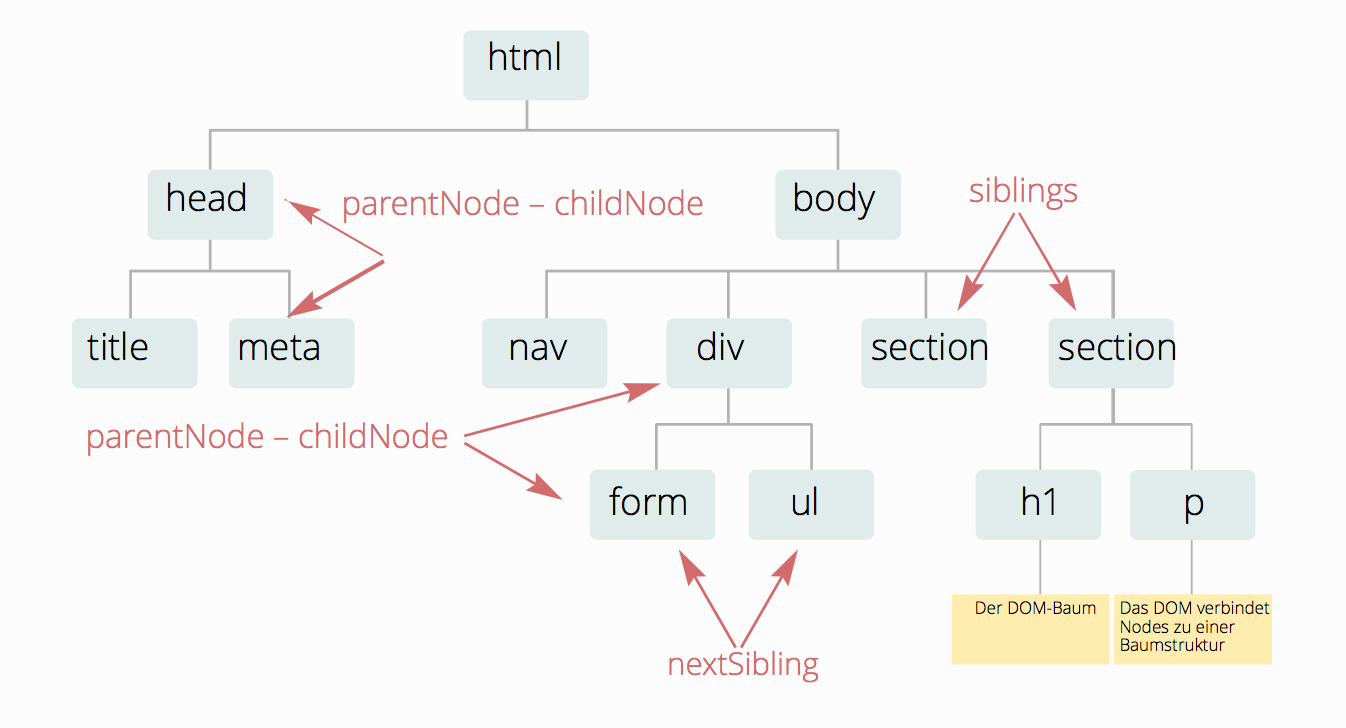
\includegraphics[width=0.7\textwidth]{imports/HTML}
  \caption{Aufbau eines HTML-Dokuments \cite{dom.html}}
\end{figure}









%%%%%%%%%%%%%%%%%%%%%%%%%%%%%%%%%%%%%%%%%%%%%%%%%%%%%%%%%%
%%%%%%%%%%					CSS					%%%%%%%%%%
%%%%%%%%%%%%%%%%%%%%%%%%%%%%%%%%%%%%%%%%%%%%%%%%%%%%%%%%%%
\section{CSS}
\label{sec:CSS}
%%%%%%%%%%%%%%%%%%%%%%%%%%%%%%%%%%%%%%%%%%%%%%%%%%%%%%%%%%

%%%%%%%%%%%%%%%%%%%%%%
\begin{description}
	\item[Die Definition und Bedeutung von CSS]
    \hfill 
    \label{des:Def_CSS}
\end{description}
%%%%%%%%%%%%%%%%%%%%%%
%
Die Seitenbeschreibungssprache \ac{HTML} dient zusammenfassend dem grundsätzlichen Aufbau der Website und definiert somit den Content. Standardmäßg werden allerdings die einzelnen \ac{HTML} Elemente nur untereinander aufgereiht und besitzen nur wenige, von dem Browser vorgegebene Formatierungen. Hier schafft\ac{CSS} Abhilfe, auf das in diesem Abschnitt eingegangen wird. So ist es eine Formatierungs- und Gestaltungssprache, mit der man fähig ist, die zuvor mittels \ac{HTML} erzeugten Elemente gezielt zu platzieren, deren Farbe und Form zu verändern und die aufzubauende Website folglich nach eigenem persönlichem Geschmack zu formatieren. Die Philosophie hierfür ist eine Trennung des Aufbaus der Website in Inhalt (\ac{HTML}) und Gestaltung (\ac{CSS}) \cite{css}.

%%%%%%%%%%%%%%%%%%%%%%
\begin{description}
	\item[Der Aufbau eines Stylesheets - Verwendung der \ac{CSS}-Regeln]
    \hfill
    \label{des:Aufbau_CSS}
\end{description}
%%%%%%%%%%%%%%%%%%%%%%
%
Der Aufbau des Stylesheets erfolgt durch die Festlegung der \ac{CSS} Regeln. Diese definieren jeweils die Formatierung eines \ac{HTML} ELements. So erfolgt der Aufbau durch eine Voranstellung eines Selektors und eines darauf folgenden Deklarators. Ersteres wählt das gewünschte, zu formatierende \ac{HTML} Element aus, zum Beispiel durch die Verwendung eines <p> Tags. Davon gibt zweiteres die Art und Weise an. Diese wird von geschweiften Klammern umgeben und enthält,von einem Doppelpunkt getrennt, zuerst die Eigenschaft und dann den Wert \cite{css-lernen}.

\newpage
%%%%%%%%%%%%%%%%%%%%%%
\begin{description}
	\item[Die diversen Arten der Selektoren - Tags, IDs und Klassen]
    \hfill
	\label{des:Selektoren_CSS}
\end{description}
%%%%%%%%%%%%%%%%%%%%%%
%
Im Folgenden wird die mögliche Verwendung von Selektoren beschrieben. Diese können entweder Tags, IDs oder Klassen sein. \textit{Tag-Selektoren} wählen, wie der Name sagt, alle Tags einer Art aus. Der \textit{ID-Selektor} wird verwendet, um einzelnen \ac{HTML} Elementen Eigenschaften zu zuweisen. Dieser wird durch das Hashtag Symbol begonnen und darauf folgend ist die \textit{HTML-ID}. Die definierten Eigenschaften gelten nun nur für das spezifische Element mit der identischen ID. 
Wenn\ac{HTML} Elemente, die mehrere, bzw. unterschiedliche Tags besitzen, nach gleichem Style formatiert werden sollen, muss auf \textit{Klassen-Selektoren} zurück gegriffen. Diese werden mit einem anfänglichem Punkt und dem Klassennamen definiert. 

\begin{table}
  \centering
  \begin{tabular}{|l|l|} \hline
  Externe Stylesheets    & Definition der Regeln in externer Formatvorlage          \\ \hline
  Inline Styles          & Direktes Festlegen der Regeln in öffnendem Tag der Datei \\ \hline
  Styles im Head Bereich & Definition der Regeln im Kopf Bereich der \ac{HTML} Datei \\ \hline
  \end{tabular}
  \label{tab:Integrationsmöglichkeiten}
  \caption{Integrationsmöglichkeiten von \ac{CSS} in \ac{HTML}}
\end{table}

%%%%%%%%%%%%%%%%%%%%%%
\begin{description}
	\item[Die Verwendung von externen Stylesheets]
    \hfill
    \label{des:Aufbau_CSS}
\end{description}
%%%%%%%%%%%%%%%%%%%%%%
%
Es gibt verschiedene Integrationsmöglichkeiten von \textit{CSS} in die \textit{HTML} Datei. Im Zuge der Arbeit wird allerdings nur auf die in dem Projekt angewandte Möglichkeit der Benutzung von externen Stylesheets eingegangen. Hier wird die Formatierung und Gestaltung in einer externen Datei ausgelagert. Die direkte Verknüpfung erfolgt dann mit einem <link> Tag. Dieses muss immer im Head der \ac{HTML} Datei stehen und verlangt zwei Attribute. Zum einem \textit{rel}, was die Beziehung des verlinkten Dokuments zur \ac{HTML} Datei angibt. Zum Anderen \textit{href}, das die URL zum verlinkten Dokument mitgibt. Der Vorteil der Verwendung von einem externen Stylesheet ist die erhöhte Flexibilität des Websitenstyles und die gesteigerte Effizienz, da diese gestaltungsgebende Datei nach Bedarf leicht ausgetauscht und zudem für mehrere \ac{HTML}-Dateien verwendet werden kann \cite{kaskade}.

\lstinputlisting[language=HTML, firstline=9, lastline=9, firstnumber=9]{src/main.html}



%%%%%%%%%%%%%%%%%%%%%%
\begin{description}
	\item[Die Gestaltung des Seitenlayouts]
	\hfill 
    \label{des:Layout_CSS}
\end{description}
%%%%%%%%%%%%%%%%%%%%%%
%
In \ac{CSS} können \ac{HTML}-Elemente grundsätzlich in zwei Arten unterteilt werden: Block- und Inline Elemente. Erstere sind klar abgegrenzte Bereiche, da sie vor und hinter sich einen Zeilenumbruch bewirken und als rechteckige Boxen dargestellt werden. Deren Breite, Höhe oder Abstand kann man beliebig festlegen. Die Darstellung von dieser Elementart und Zusammenfassung in einem Layout erfolgt über das Box-Modell.(vgl.Abb.2.2) Mit diesem kann das Layout in 4 Bereiche differenziert werden und hilft so zu einem übersichtlichen Seitenlayout Entwurf. 
%
\begin{figure}
  \centering
  
\includegraphics[width=0.7\textwidth]{imports/boxmodell.png}
  \caption{Das Box-Modell \cite{boxmodell}}
\end{figure}
%
Inline Elemente hingegen erzeugen keinen Zeilenumbruch, somit kann man zum Beispiel einzelne Wörter als solche festlegen. Die Maße sind folglich nicht individuell setzbar, sondern automatisch so lang wie das Wort. 










%%%%%%%%%%%%%%%%%%%%%%%%%%%%%%%%%%%%%%%%%%%%%%%%%%%%%%%%%%
%%%%%%%%%%			JavaScript					%%%%%%%%%%
%%%%%%%%%%%%%%%%%%%%%%%%%%%%%%%%%%%%%%%%%%%%%%%%%%%%%%%%%%
\section{JavaScript}
\label{sec:JavaScript}
%%%%%%%%%%%%%%%%%%%%%%%%%%%%%%%%%%%%%%%%%%%%%%%%%%%%%%%%%%

%%%%%%%%%%%%%%%%%%%%%%
\begin{description}
	\item[ Die Intention der Verwendung von Javascript]
    \hfill
    \label{des:Intention_JS}
\end{description}
%%%%%%%%%%%%%%%%%%%%%%
%
Für eine Websitenprogrammierung wird  neben dem Wissen über \ac{CSS} und \ac{HTML} auch ein Repertoire an verfügbarem Javascript Know-How benötigt. JavaScript wirdin eine \ac{HTML} Datei eingebunden und man ist mit Hilfe diesem Werkzeug in der Lage, beliebigen Text in einer schon dargestellten Website zu ändern. Dies ist beispielsweise bei einer immer aktuellen Anzeige der Uhrzeige auf der Website notwendig. Außerdem können dynamische Charakteristika, wie etwa das Öffnen oder Schließen von Optionen/Dateien, durch Javascript gesteuert werden \cite{javascript}.


%%%%%%%%%%%%%%%%%%%%%%
\begin{description}
	\item[Das Einbinden in das \ac{HTML}-Dokument ]
	\hfill
    \label{des:Einbindung_JS}
\end{description}
%%%%%%%%%%%%%%%%%%%%%%
%
Implementiert wird Javascript mit dem Kommando \textit{<Script>} und beendet mit \textit{</script>}, in diesem Bereich können Aufforderungen über die Dynamik der Website definiert werden. Dies kann durch einen direkten Aufruf oder über eine Einbindung einer externen Script Datei geschehen \cite{javascript}.


\newpage
%%%%%%%%%%%%%%%%%%%%%%
\begin{description}
	\item[AngularJS im Rahmen der Anwendung von Javascript]
    \hfill
    \label{des:AngularJS}
\end{description}
%%%%%%%%%%%%%%%%%%%%%%
%
Eine Option für ein JavaScript ist Angular JS. Es ist OpenSource von Google entwickelt worden. Es vereinfacht unter Anderem den Datenaustausch zwischen Frontend und Logik. Deswegen wird im folgenden auf dieses Javascript Webframework eingegangen, da es eine wichtige Rolle für die Umsetzung des Projektes spielt.
Mit AngularJs werden Direktiven, sogenannte \textit{ng-directives} in die \ac{HTML}-Datei eingebunden. Dadurch können Eingaben des Websitenbesuchers übernommen werden. Die Direktive \textit{ng-model} verbindet eine Variable mit dem Frontend. Diese kann eine Eingabe des Nutzers entgegen nehmen oder auf der Website ausgegeben werden. Diese zwei Direktiven sind die grundlegendsten Arten. Auf die in dem Projekt tatsächlich verwendeten Direktiven wird später eingegangen. 
An dieser Stelle ist die Unterscheidung der AngularJS Applikationen in die sogenannten \textit{modules} und \textit{controllers} wichtig. Ersteres definiert die AngularJS Applikation \cite{angularjs}.
\hfill
Beispielcode:

\begin{lstlisting}[language=JavaScript]	
	var applikation = angular.module('myapplikation', []);
\end{lstlisting}

Der \textit{controller} steuert einen Teil der Applikation. In folgendem Beispielcode besitzt er den Namen \textit{myController}. AngularJS ruft den Controller mit einem \textit{scope} Objekt auf. In diesem legt der \textit{controller} zwei Variablen an: \textit{firstName} und \textit{lastName}. 

\begin{lstlisting}[language=JavaScript]	
app.controller('myCtrl', function($scope) {
    $scope.firstName = "Max";
    $scope.lastName = "Muster";
});
\end{lstlisting}

Dies ist das grundlegende Wissen, das für die Durchführung des Projektes benötigt wird. 

















\chapter{Projektdurchführung}
\label{cha:Projektdurchführung}


%%%%%%%%%%%%%%%%%%%%%%%%%%%%%%%%%%%%%%%%%%%%%%%%%%%%%%%%%%
%%%%%%%%%%			Latex Vorlage				%%%%%%%%%%				
%%%%%%%%%%%%%%%%%%%%%%%%%%%%%%%%%%%%%%%%%%%%%%%%%%%%%%%%%%
\section{Erstellen der Latex Vorlage}
\label{sec:Aufbau_HTML}
%%%%%%%%%%%%%%%%%%%%%%%%%%%%%%%%%%%%%%%%%%%%%%%%%%%%%%%%%%
\begin{figure}[H]
   	\centering
   	\fbox{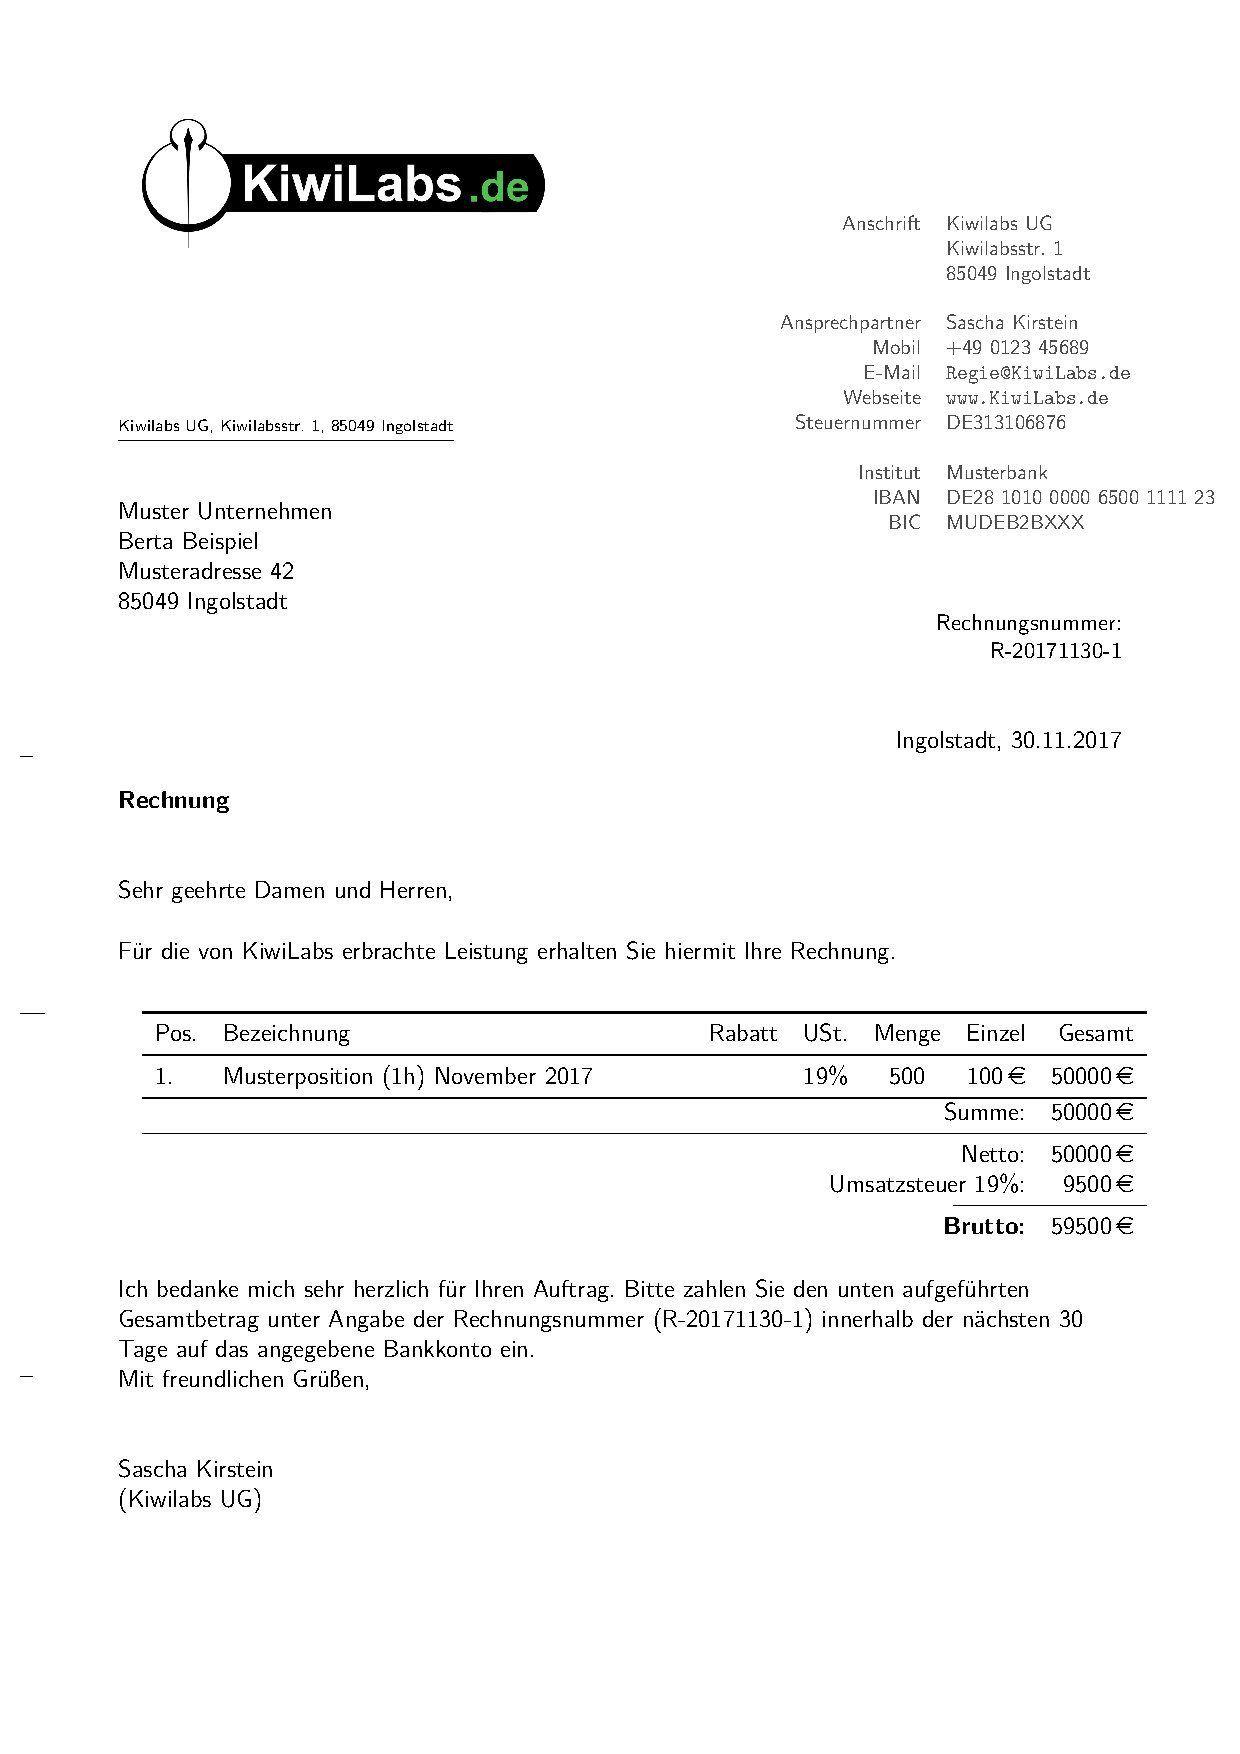
\includegraphics[width=0.7\textwidth]{imports/muster-unternehmen-rechnung}}
   	\caption{Die fertige Kiwilabs-Rechnungsvorlage}
\end{figure}

Im ersten Schritt wird das Latex Dokument erstellt. Die Grundlage bildet dabei die Briefklasse \textit{scrlttr2} aus dem KOMA-Script. Bestimmte Stellen müssen am Ende aus der Java Anwendung verändert werden. Diese Textstellen werden zur verbesserten Strukturierung nicht in der zentralen Latex-Datei, sondern in der \textit{Data.tex} Datei zur Trennung des festen Layouts und der veränderlichen Dateien ausgelagert. Dafür wird die Funktion \bashCommand{\textbackslash newcommand} verwendet, um die Textbreiche in der Vorlage durch Werte in der \textit{Data.tex} zu ersetzen. In diesem Beispiel \bashCommand{\textbackslash newcommand\{\textbackslash senderCompany\}\{KiwiLabs UG\}} wird in \textit{Data.tex} das Kommando \bashCommand{\textbackslash senderCompany} definiert.  In der Vorlage wird anstelle des festen Werts "`KiwiLabs UG"` der neue Befehl aufgerufen. Soll durch das Java Programm der Wert verändert werden, reicht eine Anpassung von \textit{Data.tex} um alle Vorkommen in der Vorlage auszutauschen.


%%%%%%%%%%%%%%%%%%%%%%%%%%%%%%%%%%%%%%%%%%%%%%%%%%%%%%%%%%
%%%%%%%%%%				Webseite				%%%%%%%%%%				
%%%%%%%%%%%%%%%%%%%%%%%%%%%%%%%%%%%%%%%%%%%%%%%%%%%%%%%%%%
\section{Erstellen der Webseite}
\label{sec:Erstellen_Webseite}
%%%%%%%%%%%%%%%%%%%%%%%%%%%%%%%%%%%%%%%%%%%%%%%%%%%%%%%%%%
\subsection{Gestaltung des Frontends}
\label{subsec:Gestaltung_Webseite}
%%%%%%%%%%%%%%%%%%%%%%%%%%%%%%%%%%%%%%%%%%%%%%%%%%%%%%%%%%
Ausgehend von der Latex Vorlage sind folgende Elemente auf der Website notwendig: 
%
\begin{itemize}
	\item  Rechnungssteller mit Eingabefeld
    \item  Rechnungsempfänger mit Eingabemöglichkeiten für  	
    		\begin{itemize}
				\item den Firmennamen
            	\item den Kundennamen
            	\item und der Adresse
         	\end{itemize}   
     \item Rechnungspositionen mit 
    	 	\begin{itemize}
				\item Bezeichnung
            	\item Menge
            	\item Einzelpreis
           	    \item Rabatt
           		\item Steuern
            \end{itemize}  
     
	\item Button für die Erstellung des Latex-Dokuments    
\end{itemize}
%
Das fertige Layout wird Schritt für Schritt in den nächsten Absätzen der Arbeit erklärt und verdeutlicht, wie der Quellcode implementiert worden ist. An dieser Stelle wird für einen Überblick das Resulat gezeigt.
%
\begin{figure}[H]
    \centering
    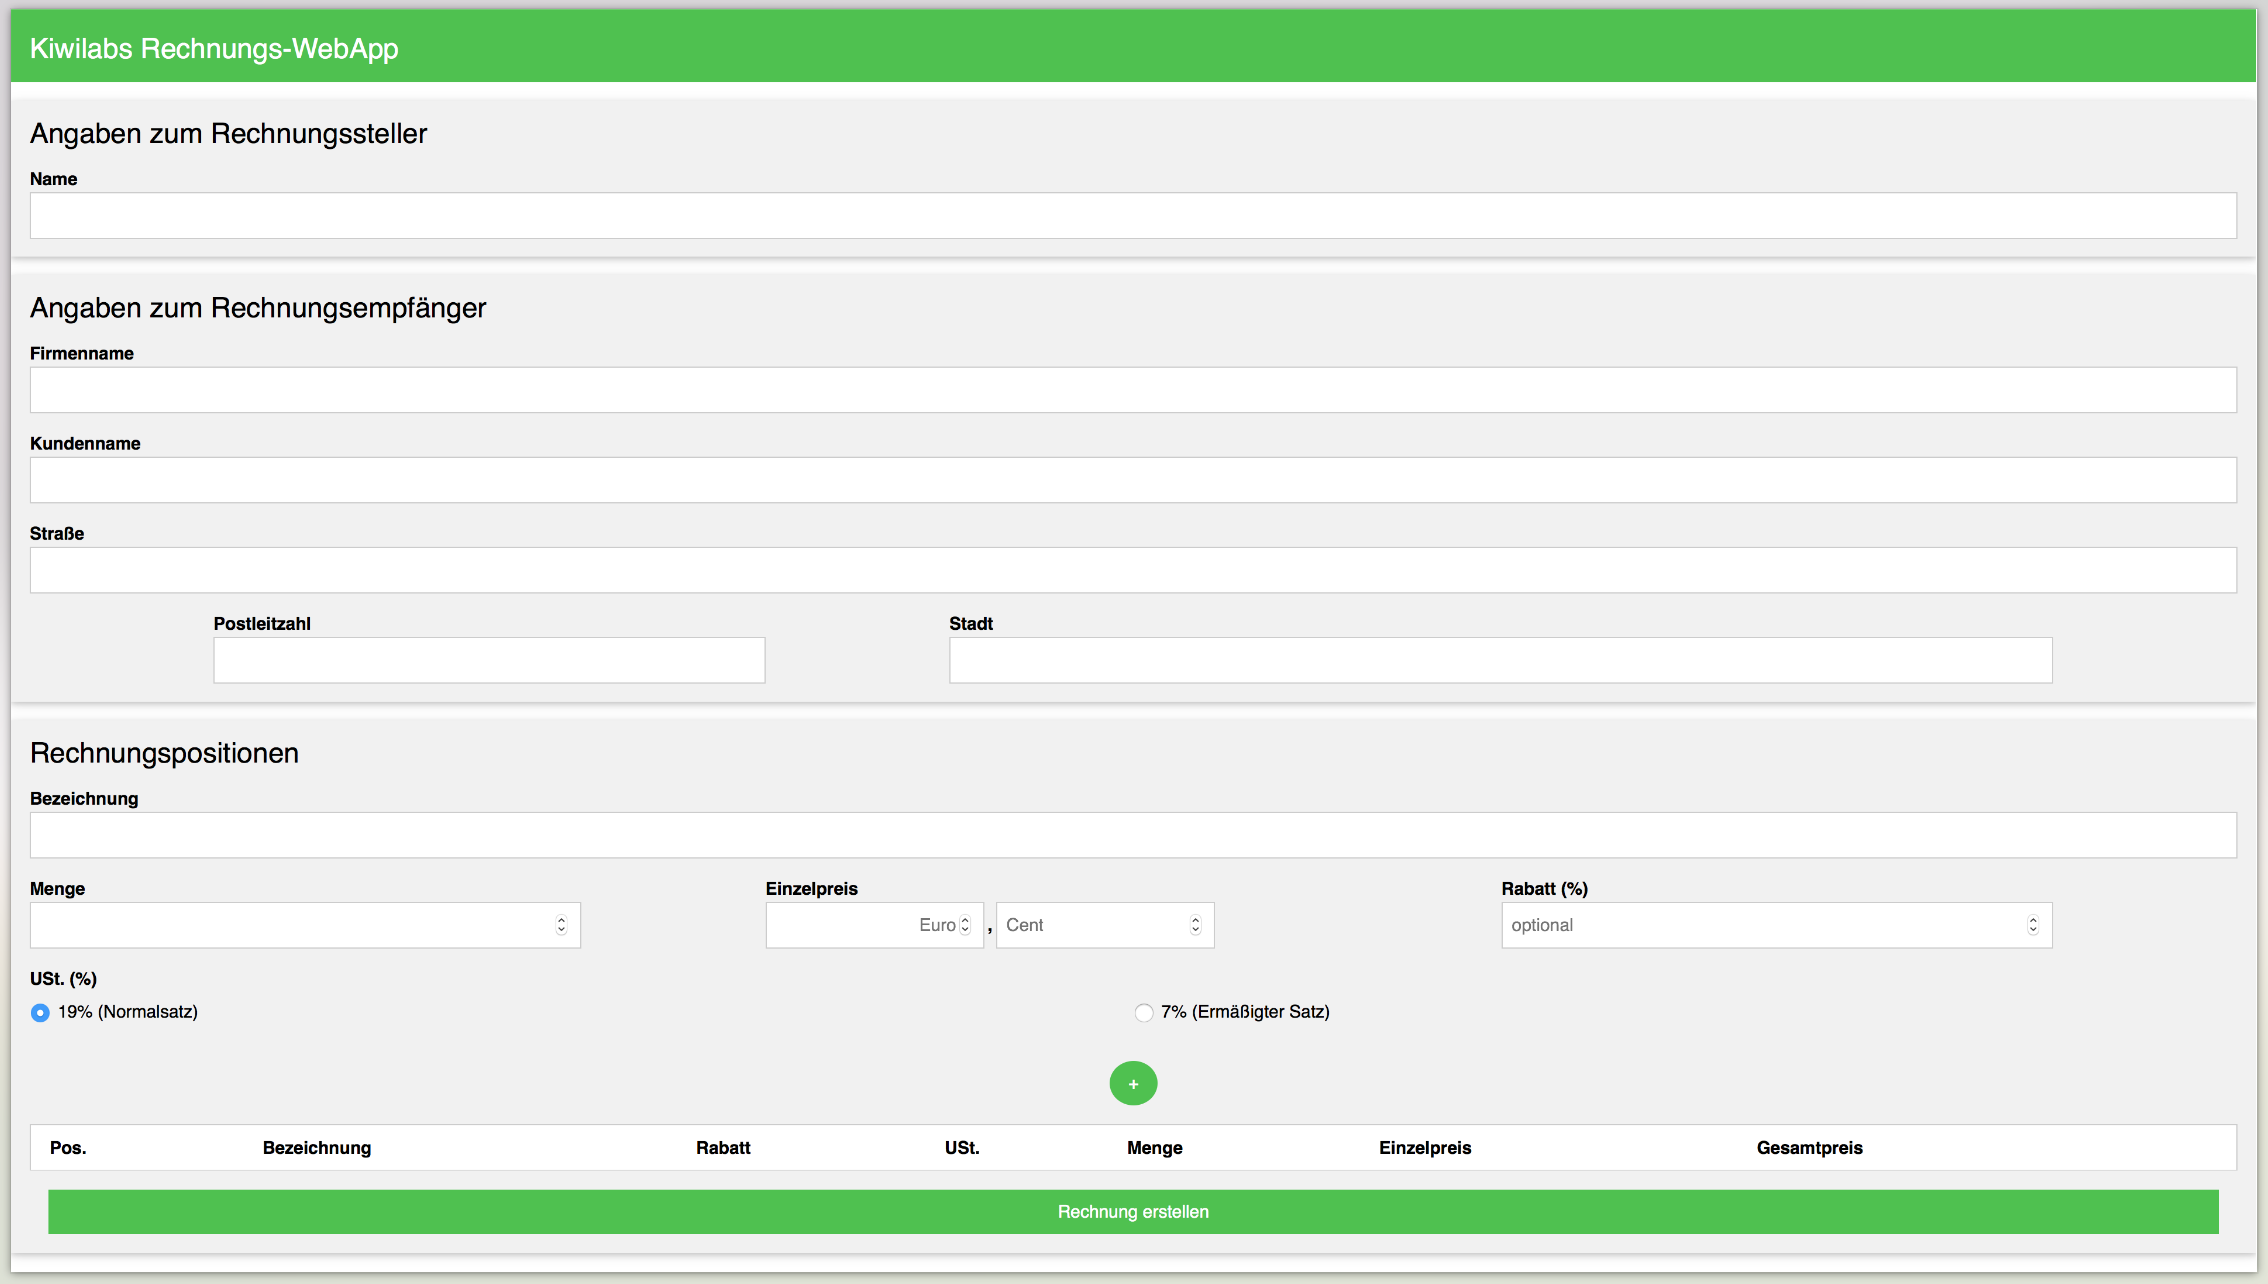
\includegraphics[width=1.0\textwidth]{imports/Layoutgesamt}
    \caption{Vollständiges Layout der Website}
\end{figure}
%
Ausgehend von den \ac{HTML}-Kenntnissen (siehe Seite \pageref{sec:HTML}) wird der \textit{Head} des Dokuments angelegt.
\lstinputlisting[language=HTML, firstline=1, lastline=14, firstnumber=1]{src/main.html} \label{Head} 

In Zeile 9 wird ein externes Stylesheet\cite{w3.css} eingebunden. Diese Vorlage ist lizenzfrei verfügbar von w3. Der \textit{Body} des HTML-Dokuments wird in Zeile 14 begonnen.\ref{Head}

\newpage
%%%%%%%%%%%%%%%%%%%%%%
\begin{description}
	\item[Angaben zum Rechnungssteller]
    \hfill
    \label{des:Angaben_Rechnungssteller}
\end{description}
%%%%%%%%%%%%%%%%%%%%%%
%
\lstinputlisting[language=HTML, firstline=22, lastline=39, firstnumber=22]{src/main.html}

In Zeile 22 wird ein neuer \textit{div}-Tag mit der Klasse \textit{w3-card} eröffnet. Dies ist eine Box mit Schatteneffekt. In Zeile 24 wird ein neuer div-Tag geöffnet, der ein Container mit einem Padding von 16 Pixel mit der Hintergrundfarbe von hellgrau darstellt. Dieses Element hat die schwarze Überschrift \textit{Angaben zum Rechnungssteller}. 
\begin{figure}[H]
    \centering
    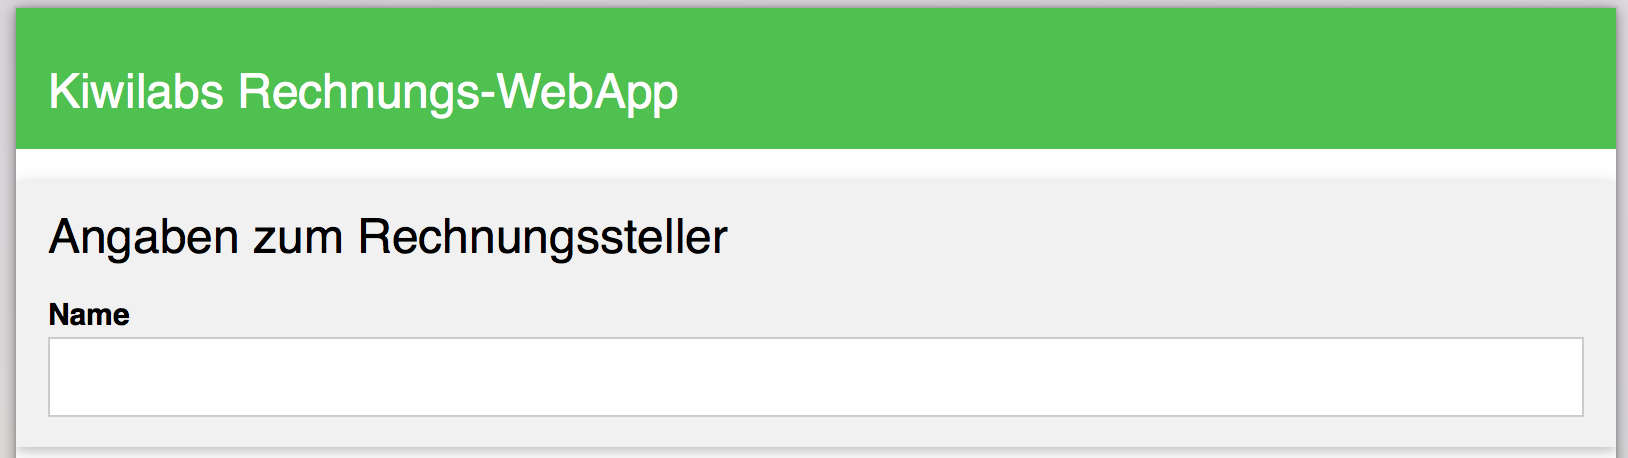
\includegraphics[width=0.7\textwidth]{imports/AzR}
    \caption{  Angaben zum Rechnungssteller}
  
\end{figure}
%
Ab Zeile 27 wird der Input beschrieben. Die darauf folgenden Attribute \textit{ng-click} und \textit{ng-model} sind Elemente von AngularJs, die die Reaktion der Eingabefelder gewährleisten. Dieser Punkt wird später näher beschrieben. \textit{w3-input} ist die Definition für einen Input und \textit{w3-border} sorgt für eine Umrandung des HTML-Elements. Zur korrekten Vervollständigung wurde außerdem eine ID, ein Name und ein Typ angegeben.
Der nächste Bereich, eingeleitet durch den Aufruf \textit{div} in Zeile 29, dient zur Implementierung des PopUp Effekts für eine Schnellauswahl der Rechnungssteller. Die Elemente dieser werden durch eine ungeordnete Liste, abgekürzt durch \textit{ul}, dargestellt. \textit{w3-hoverable} sorgt für die dynamische Hervorhebung des Namens, wenn die Maus des Nutzers über die Stelle fährt. 

\newpage
%%%%%%%%%%%%%%%%%%%%%%
\begin{description}
	\item[Angaben zum Rechnungsempfänger]
    \hfill
     \label{des:Angaben_Rechnungsempfänger}
\end{description}
%%%%%%%%%%%%%%%%%%%%%%
%
Die Layouterstellung des Abschnittes über die \textit{Angaben zum Rechnungsempfänger} sind analog zu \textit{Angaben zum Rechnungssteller}, weswegen nicht näher darauf eingegangen wird.


%%%%%%%%%%%%%%%%%%%%%%
\begin{description}
	\item[Darstellung der Rechnungspositionen]
    \hfill
    \label{des:Rechnungspositionen}
\end{description}
%%%%%%%%%%%%%%%%%%%%%%
%
Der Abschnitt zu den Rechnungspositionen wird in Zeile 88 begonnen. In Zeile 98 beginnt eine \textit{w3-row}. Diese sorgt für eine Reihung der Elemente \textit{Menge}, \textit{Einzelpreis} und \textit{Rabatt} nebeneinander. Für den Anwender soll das Layout nicht nur in der Ansicht eines Laptops oder PC, sondern auch in einer mobilen Version ansehnlich sein. Dies wird in Zeile 101 mittels der Klasse \textit{w3-col} gewährleistet. \textit{m3} definiert die Darstellung für alle Medium Geräte, diese sind bei \textit{w3school} größer als 601 Pixel. In dieser Darstellung nimmt es 3/12 der Bildschirmbreite ein. Ein Endgerät mit weniger als 601 Pixel Bildschirmbreite wird von \textit{w3.css} als \textit{small} bezeichnet. Dieses würde in diesem Fall das Element auf der gesamten Bildschirmbreite angezeigt bekommen. In Zeile 106 wird der Abstand zwischen den Feldern \textit{Menge} und \textit{Einzelpreis} bei großen Bildschirmen eingefügt. Der Aufruf \textit{w3-hide-small} entfernt den Abstand in der Ansicht von kleinen Bildschirmen.

\begin{figure}[H]
    \centering
    \begin{minipage}{0.45\linewidth}
        \centering
        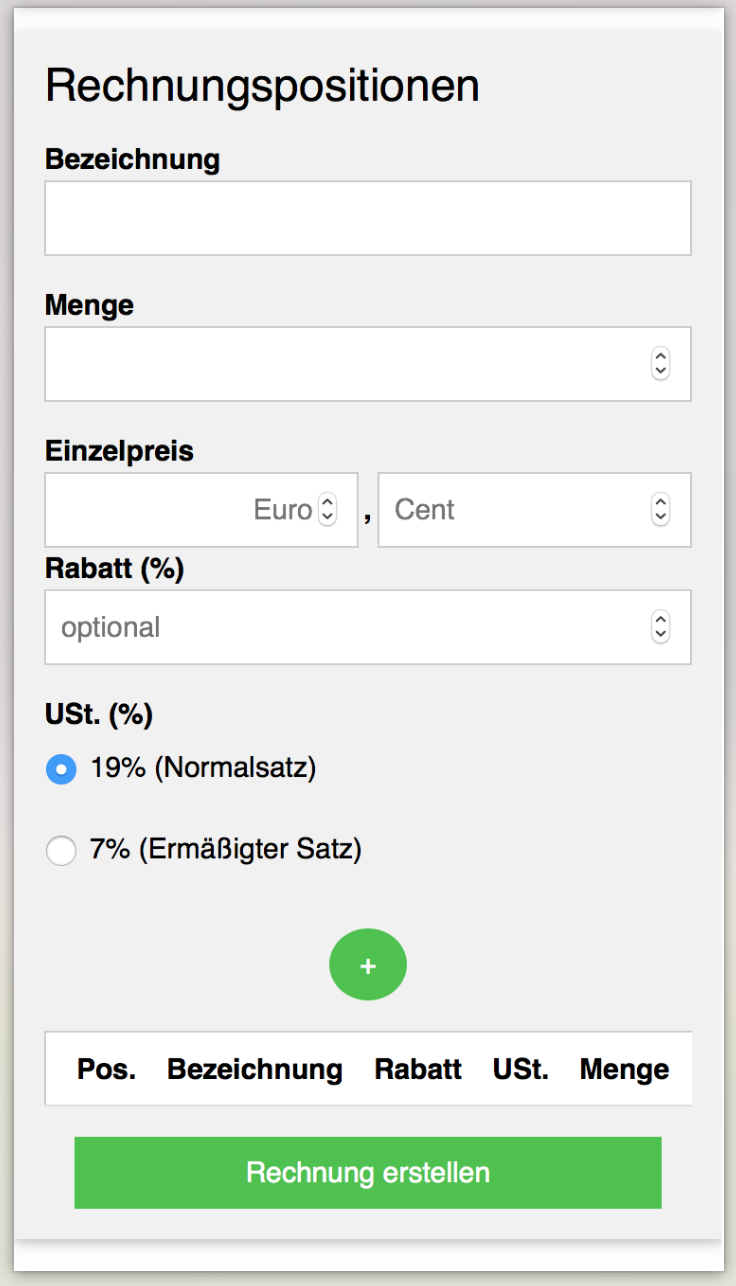
\includegraphics[width=0.33\textwidth]{imports/smallView}
        \caption{Mobile Ansicht}
    \end{minipage}
    %\hfill
    \begin{minipage}{0.45\linewidth}
        \centering
        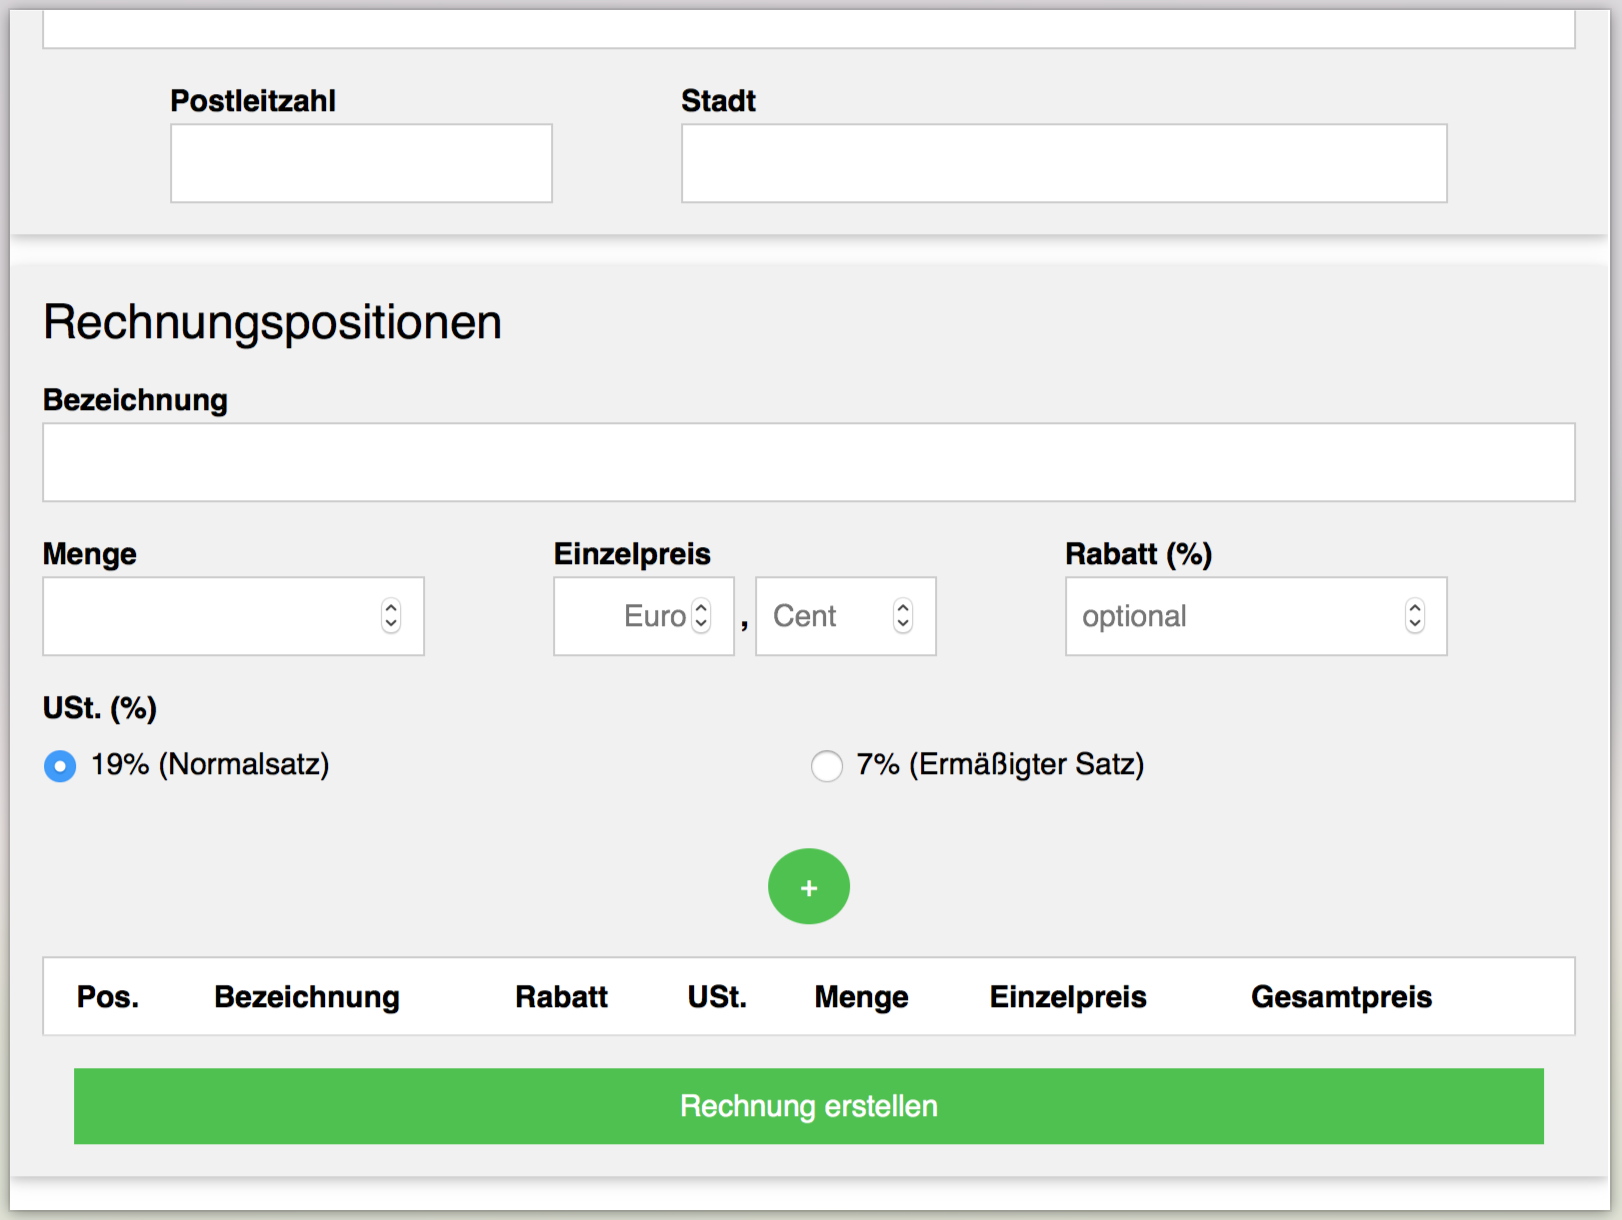
\includegraphics[width=0.8\textwidth]{imports/medium+largeView}
        \caption{Desktop Ansicht}
    \end{minipage}
\end{figure}

\lstinputlisting[language=HTML, firstline=88, lastline=108, firstnumber=88]{src/main.html}

Das Feld für den Einzelpreis wird ab Zeile 111 definiert, welches in Euro und Cent dargestellt werden soll, um den individuellen Kostenbetrag darstellen und eine weitere Verarbeitung des Betrages erreichen zu können. Wenn der Kostenbetrag mit Kommatrennung des Euro- und Centanteils in ein Feld geschrieben werden würde, müsste dieser mit einer Parse-Funktion eventuell später überarbeitet werden. Dieser Schritt wird durch eine explizite Trennung in zwei Eingabefelder eingespart. Diese beiden Felder werden jeweils durch eine \textit{w3-cell} definiert, diese ist ein einfaches und horizontal orientiertes Block-Element. 
Auf die Eingabefunktion und Übernahme des Betrages zu einem späteren Zeitpunkt eingegangen.

\lstinputlisting[language=HTML, firstline=111, lastline=129, firstnumber=111]{src/main.html}

Das nächste Feld der Rechnungspositionen ist der Rabatt, dies wird in der Zeile 132 begonnen und in Zeile 137 mit \bashCommand{</div>} beendet.

\lstinputlisting[language=HTML, firstline=132, lastline=137, firstnumber=132]{src/main.html}

Das letzte Element für die Rechnungspositionen ist die zu addierende Umsatz- und Mehrwertsteuer, die in der Preisberechnung berücksichtigt werden muss. 
Hier wird wieder eine \textit{w3-row} eröffnet, die mit USt. und 7 Prozent Ermäßigter Satz beschriftet wird. Dazwischen befinden sich Elemente, die durch AngularJs interaktiv auf den Nutzer der Website reagieren.

\lstinputlisting[language=HTML, firstline=141, lastline=152, firstnumber=141]{src/main.html}

Um weitere Positionen hinzufügen zu können, ist eine Add-Funktion gefordert, die benutzerfreundlich durch einen Plus-Button repräsentiert wird. 
%
Als letzter Punkt soll in der Ansicht der Website in einer Zeile alle Punkte der Rechnung übersichtlich dargestellt sein, was nun definiert wird. In Zeile 154 wird hierzu das Element in dem Zentrum des Bildschirms angeordnet. Innerhalb des \textit{ng-click} von AngularJS wird das Feld als runder Button mit grüner Füllung und automatisch berechnetem Abstand. 

\lstinputlisting[language=HTML, firstline=154, lastline=156, firstnumber=155]{src/main.html}

\begin{figure}[H]
    \centering
    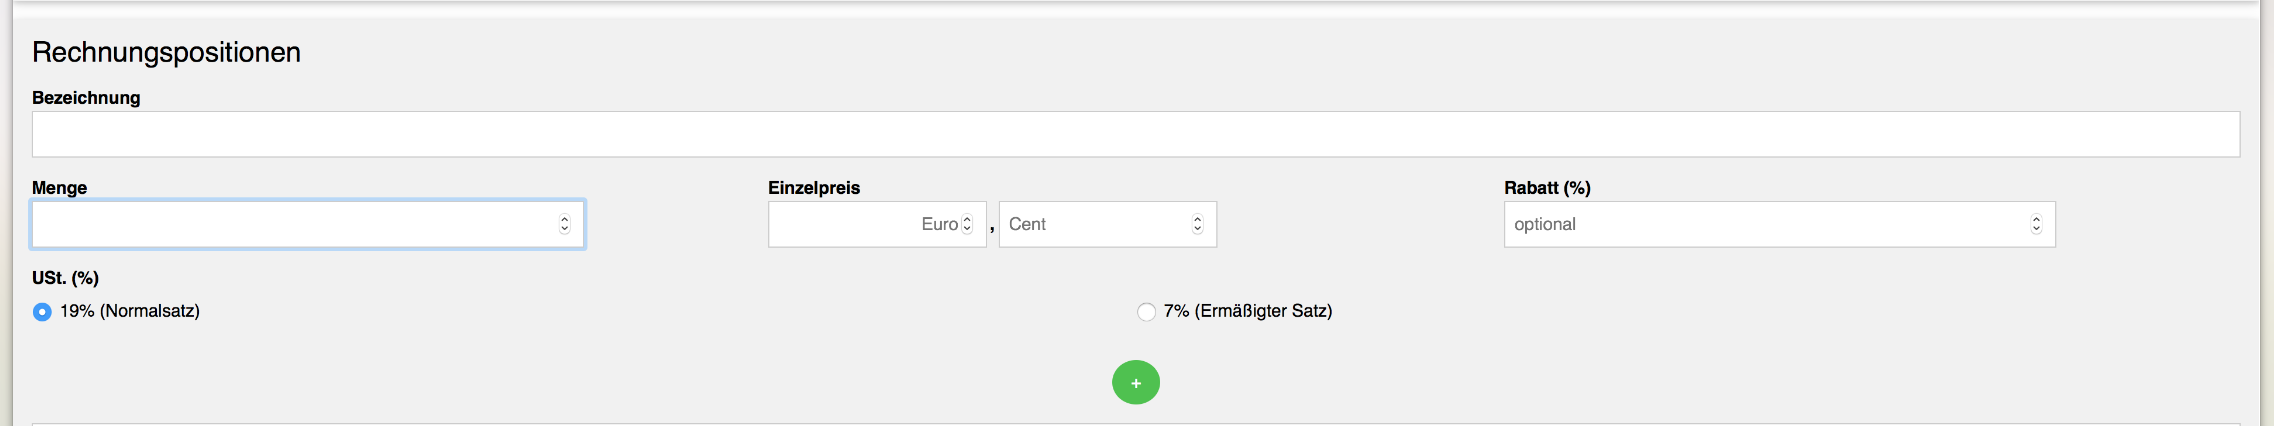
\includegraphics[width=0.7\textwidth]{imports/Rechnungspositonen}
    \caption{ Fertige Ansicht der Rechnungspositionen}
\end{figure}
%
Nun sind die benötigten Punkte der Rechnungspositonen komplettiert und zur Veranschaulichung der gesamten Rechnung werden am Ende des Websitenlayouts alle Teile in einer Reihe aufgeführt. 
\\

Für diese Anforderung wird eine Tabelle eröffnet, die sich dynamisch an die jeweilige Bildschirmgröße anpasst. ( \textit{w3-responsive, Z. 158f}. Die einzelnen Punkte werden in der Tabelle durch den \bashCommand{<t>} Tag in Zeile 160 und die jeweiligen \bashCommand{<th>} Tags als einzelne Elemente in einer neuen Zeile implementiert.

\lstinputlisting[language=HTML, firstline=158, lastline=182, firstnumber=158]{src/main.html}


%%%%%%%%%%%%%%%%%%%%%%
\begin{description}
	\item[Button für die Erstellung des Latex-Dokuments]
    \hfill
    \label{des:AddButton}
\end{description}
%%%%%%%%%%%%%%%%%%%%%%
%
Der Button für die Erstellung des Latex-Dokuments wird zentriert auf dem Display des Nutzers (vgl. Z.184 ) platziert. Außerdem ist der \textit{w3-button} ein grüner Block, weswegen er die gesamte Breite des Bildschirms benutzt und die Aufschrift \glqq{\textit{Rechnung erstellen}} trägt. Die Erstellung in ein pdf wird über AngularJs in \textit{Logik des Frontends} gewährleistet.



%%%%%%%%%%%%%%%%%%%%%%%%%%%%%%%%%%%%%%%%%%%%%%%%%%%%%%%%%%
%%%%%%%%%%				Logik					%%%%%%%%%%	
%%%%%%%%%%%%%%%%%%%%%%%%%%%%%%%%%%%%%%%%%%%%%%%%%%%%%%%%%%
\subsection{Logik des Frontends}
\label{sec:Logik}
%%%%%%%%%%%%%%%%%%%%%%%%%%%%%%%%%%%%%%%%%%%%%%%%%%%%%%%%%%


%%%%%%%%%%%%%%%%%%%%%%
\begin{description}
	\item[Logik für Rechnungssteller und -empfänger]
    \hfill
    \label{des:Logik}
\end{description}
%%%%%%%%%%%%%%%%%%%%%%
%
Die Logik des Frontends ist ein substantieller Teil der Websitencharaktertistik. Durch diese wird die Reaktion der Website auf Benutzereingaben oder Veränderungen der Fenstergröße garantiert. 
%
AngularJS wird das erste Mal in dem Projekt benötigt, wenn bei der Auswahl des Rechnungsstellers zwischen zuvor hinterlegten Personen gewählt werden soll, die als neue Option auf dem Desktop erscheinen sollen. Eine solche Interaktion wird in Zeile 27 durch den \textit{input}-Aufruf \textit{ng-click} und \textit{ng-model} implementiert.  Die erste Direktive teilt dem Java-Framework AngularJs mit, was bei einem Klick des Nutzers geschehen soll. Dies ist in diesem Fall \textit{toggleSenderList()}, diese Funktion wird in \textit{invoiceApp.js} definiert. Die Direktive \textit{ng-model} verbindet das Eingabefeld mit der in \textit{invoiceApp.js} definierten Variable\textit{senderName}. \textit{ng-show} ermöglicht die Darstellung der Sender Liste. Die Namen werden über die REST Schnittstelle im JSON Format übergeben und dienen der Vorauswahl. Wenn neue Namen eingeben werden, die noch nicht existent sind, werden diese an den Server übergeben und hinterlegt.
Die Logik für die Auswahl der Rechnungsempfänger\textit{(vgl. 48ff)} ist entsprechend diesem Prinzip. 

%%%%%%%%%%%%%%%%%%%%%%
\begin{description}
	\item[PDF-Erstellung]
    \hfill
    \label{sec:PDF}
\end{description}
%%%%%%%%%%%%%%%%%%%%%%
%
\lstinputlisting[language=HTML, firstline=184, lastline=186, firstnumber=183]{src/main.html}

In Zeile 185 des html-Dokuments wird mittels \textit{ng-click} mitgeteilt, dass bei einem Klick auf den Button \textit{downloadPDF} die gleichnamige, in \textit{invoiceApp.js} definierte Funktion ausgeführt werden soll. 
Diese legt das Objekt\textit{data} neu an und befüllt deren Variablen mit denen aus der Website. Im nächsten Schritt wird \textit{data} an den \textit{localhost} gepostet. Falls dies nicht funktioniert, wird die Nachricht "Fehler" gemeldet.

\lstinputlisting[language=JavaScript, firstline=79, lastline=99, firstnumber=79]{src/invoiceApp.js}



\chapter{Fazit und Ausblick}
\label{cha:Fazit}

Dieses Layout wurde mittels HTML, CSS und dem JavaScript Framework Angular JS umgesetzt. 
Die gestellten Anforderungen werden bis auf die Pflege gestellter Angebote und Rechnungen, sowie eine Verwaltung von Firmen mit Kontaktpersonen erfüllt. Insgesamt ist das Frontend fertig.
In den nächsten Schritten können der, bis jetzt fehlende, Webserver und eine Datenbank, die mithilfe von SQL verwirklicht werden kann, aufgesetzt werden. Auch die Java-Applikation für eine Datenannahme der Kundeninformationen und die anschließende Verarbeitung zur Ausgabe einer pdf-Datei ist angedacht, dessen Grundfunktion bereits implementiert ist. Nach dieser Umsetzung werden schlussendlich alle gestellten Anforderungen erfüllt.
%\lstinputlisting[language=HTML]{src/main.html}

%\lstinputlisting[language=JavaScript]{src/invoiceApp.js}

%\lstinputlisting{src/data.tex}



\chapter*{Literaturverzeichnis}
	
	\bibliographystyle{plaindin}	% DIN Norm fuer Literaturdarstellung
\addcontentsline{toc}{chapter}{Literaturverzeichnis}
	

\begin{btSect}{ref/ref_books}
 \section{Bücher}
 \btPrintAll
\end{btSect}


\begin{btSect}{ref/ref_online}
 \section{Internetquellen}
 \btPrintAll
\end{btSect}
			
\chapter*{Abkürzungsverzeichnis}

	\begin{acronym}[ECU]
\acro{pdf}[PDF]{Portable Document Format}
\acro{CSS}[CSS]{Cascading Style Sheet}
\acro{HTML}[HTML]{Hypertext Markup Language}
\acro{http}[HTTP]{Hypertext Transfer Protocol}
\end{acronym}


%Ende Text
\end{document}